\documentclass[lualatex, aspectratio=169]{beamer}

\usetheme{Data61}

\title{Aboleth}
\subtitle{Bayesian Neural Networks and More}
\author{Dan Steinberg}
\date{April 11, 2018}
\institute{Inference Systems Engineering}

\usepackage{fontspec}
\usepackage{color}
\usepackage{unicode-math}
\usefonttheme{serif}

\defaultfontfeatures{Ligatures=TeX}
\setmainfont{Open Sans}
\setsansfont{Open Sans}
\setmonofont{Inconsolata}
% \setmathfont{DejaVu Math Tex Gyre}
% \setmathfont{XITS Math}

% Math
\renewcommand{\v}[1]{\mathbf{#1}}
\renewcommand{\d}{\,\mathrm{d}}
\newcommand{\T}{^\top}
\newcommand{\vp}[1]{\mathbf{#1}^{\prime}}
\newcommand{\h}[1]{\hat{#1}}
\newcommand{\cov}[2]{\mathrm{Cov}(#1,#2)}
\newcommand{\hil}{\mathscr{H}}
\newcommand{\reals}{\mathbb{R}}
\newcommand{\complexs}{\mathbb{C}}
\newcommand{\dprod}[2]{{\langle #1, #2 \rangle}}
\newcommand{\expec}[1]{\mathbb{E}\!\left[{#1}\right]}
\newcommand{\argmin}{\operatornamewithlimits{argmin}}
\newcommand{\pd}[2]{\frac{\partial#1}{\partial#2}}
\newcommand{\norm}[1]{\|#1\|}
\newcommand{\query}[1]{{#1}^{*}}


% Text
\newcommand{\imp}[1]{\textcolor{Data61 green}{\textbf{#1}}}

%%%%%%%%%%%%%%%%%%%%%%%
% global renew commands
%%%%%%%%%%%%%%%%%%%%%%%
\makeatletter
\def\gnewcommand{\g@star@or@long\new@command}
\def\grenewcommand{\g@star@or@long\renew@command}
\def\g@star@or@long#1{% 
  \@ifstar{\let\l@ngrel@x\global#1}{\def\l@ngrel@x{\long\global}#1}}
\makeatother
%%%%%%%%%%%%%%%%%%%%%%%%%%%
% end global renew commands
%%%%%%%%%%%%%%%%%%%%%%%%%%%

\let\oldint\int
\grenewcommand\int{\oldint\!}
\grenewcommand{\epsilon}{\varepsilon}

\let\oldemptyset\emptyset
\let\emptyset\varnothing

\newtheorem{prp}{Proposition}[section]
\newtheorem{thm}{Theorem}[section]

\theoremstyle{definition}
\newtheorem{dfn}{Definition}[section]

\newcommand{\sidenote}[1]{
  \marginline{{\fontsize{8}{8}\selectfont
    \begin{spacing}{1}
#1
    \end{spacing} }}
}



\begin{document}

\maketitle

\begin{frame}{Outline}
  \begin{itemize}
    \item Supervised learning
    \item ...
  \end{itemize}
\end{frame}

\section{Supervised learning and Neural Nets}


\begin{frame}{Supervised learning}
  \begin{itemize}
    \item <1-> $\v{x}$ is a vector of covariates, $y$ a target 
    \item <2-> There exists an unknown function, $f$, that maps the covariates to the targets,
      \begin{align*}
        y = f(\v{x}) + \epsilon
      \end{align*}
    \item <3-> \emph{Supervised ML}: learn an approximation of this function, $h$, using examples,
      \begin{align*}
        y_i \approx h(\v{x}_i) \quad \text{for all} \quad \{(y_1, \v{x}_1), (y_2, \v{x}_2), \ldots,
          (y_N, \v{x}_N) \}
      \end{align*}
  \end{itemize}
\end{frame}


\begin{frame}{Supervised learning}
  Usually we parameterise $h$ by $\theta$, and learning is often \imp{optimisation} of these parameters,
  \begin{align*}
    \hat{\theta} = \argmin_\theta \frac{1}{N} \sum^N_{i=1} \mathcal{L}\!\left(y_i, h(\v{x}_i, \theta)\right),
  \end{align*}
  where $\mathcal{L}$ is a \imp{loss} or \imp{error} function.
  % For example, linear regression,
  % \begin{align*}
  %   \argmin_{\v{w}} \frac{1}{N} \sum^N_{i=1} \|y_i - \v{w}^\top \v{x}_i \|^2_2
  % \end{align*}

\end{frame}


\begin{frame}{Prediction}
  Once we have learned $h$, we want to use it to \imp{predict} $\query{y}$ for \imp{new}, \imp{unseen} instances of $\query{\v{x}}$,
  \begin{align*}
    \expec{\query{y}} = h(\query{\v{x}}, \hat{\theta}).
  \end{align*}
  with as little \imp{error} as possible --- we want $h$ to \imp{generalise} from example!
\end{frame}


\begin{frame}{Regression Example}

  \begin{description}
    \item[True function] $f(x) = \sin(x)$
    \item[Observations] $y_i = f(x_i) + \epsilon_i, \quad \epsilon_i \sim \mathcal{N}(0, 0.1)$
  \end{description}

  \begin{figure}
    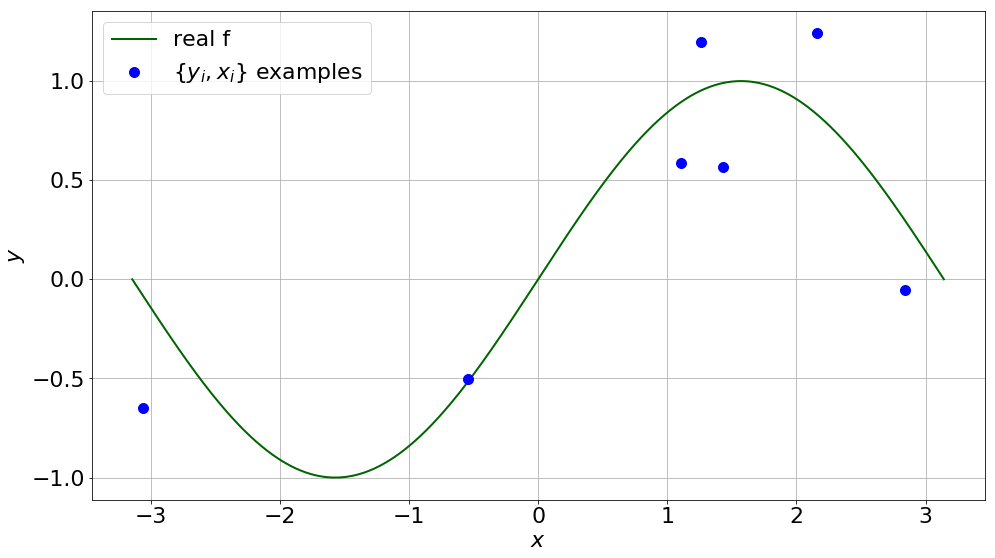
\includegraphics[width=0.5\pagewidth]{assets/regress.png}
  \end{figure}

\end{frame}


\begin{frame}{Regression Example}

  \begin{description}
    \item<1>[Model] $h(x) = w_0 + w_1 x$
    \item<2>[Model] $h(x) = w_0 + w_1 x + w_2 x^2 + w_3 x^3$
    \item<3>[Model] $h(x) = w_0 + w_1 x + \ldots + w_9 x^9$
    \item[Objective] $\argmin_{w} \frac{1}{N} \sum^N_{i=1} \|y_i - h(x_i)\|^2_2$ 
  \end{description}

  \begin{figure}
    \begin{overprint}%
      \onslide<1>\centerline{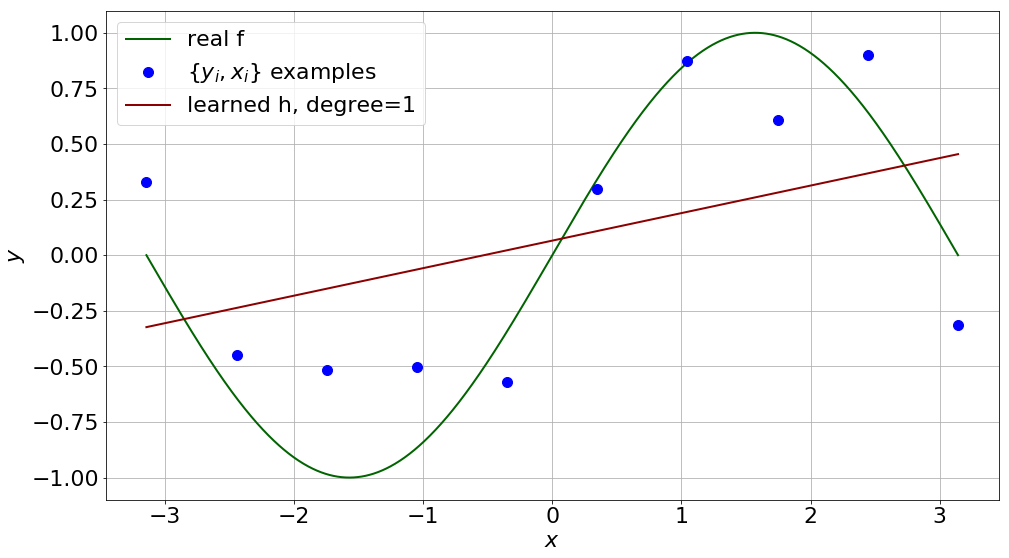
\includegraphics[width=0.5\pagewidth]{assets/poly1.png}}
      \onslide<2>\centerline{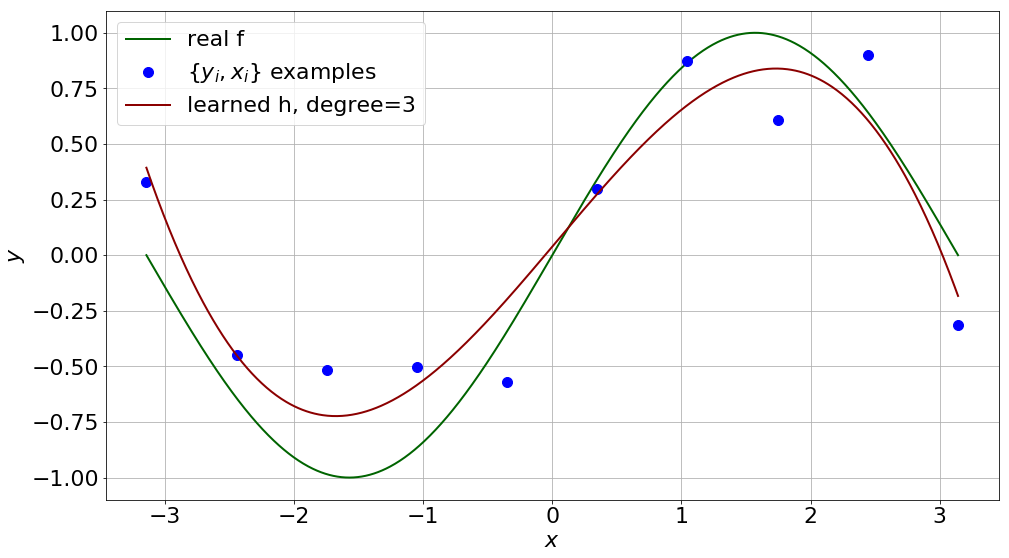
\includegraphics[width=0.5\pagewidth]{assets/poly3.png}}
      \onslide<3>\centerline{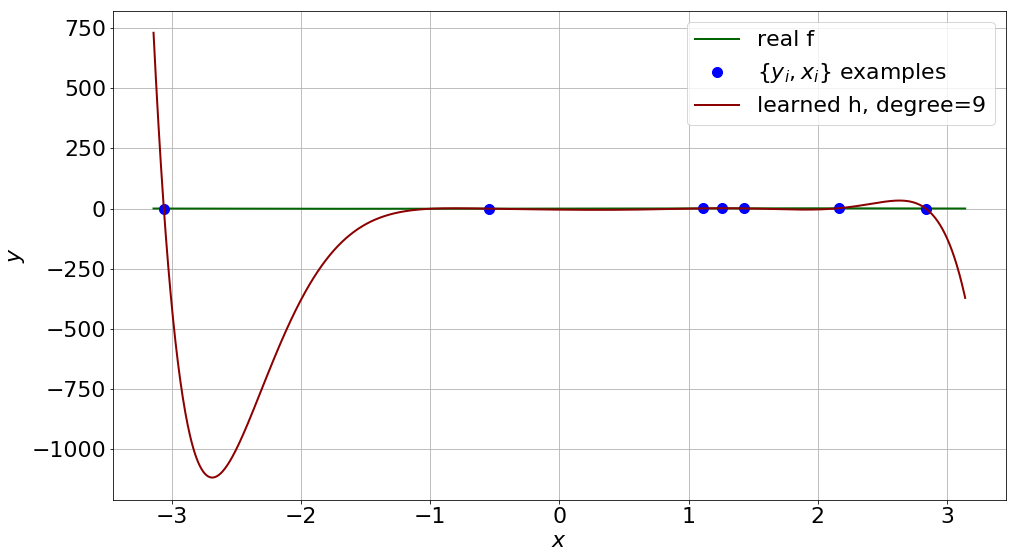
\includegraphics[width=0.5\pagewidth]{assets/poly9.png}}
    \end{overprint}
  \end{figure}

\end{frame}


% \begin{frame}{Nearest Neighbour}
%   \begin{tikzpicture}[remember picture, overlay]
%             \node[at=(current page.center)] {
%   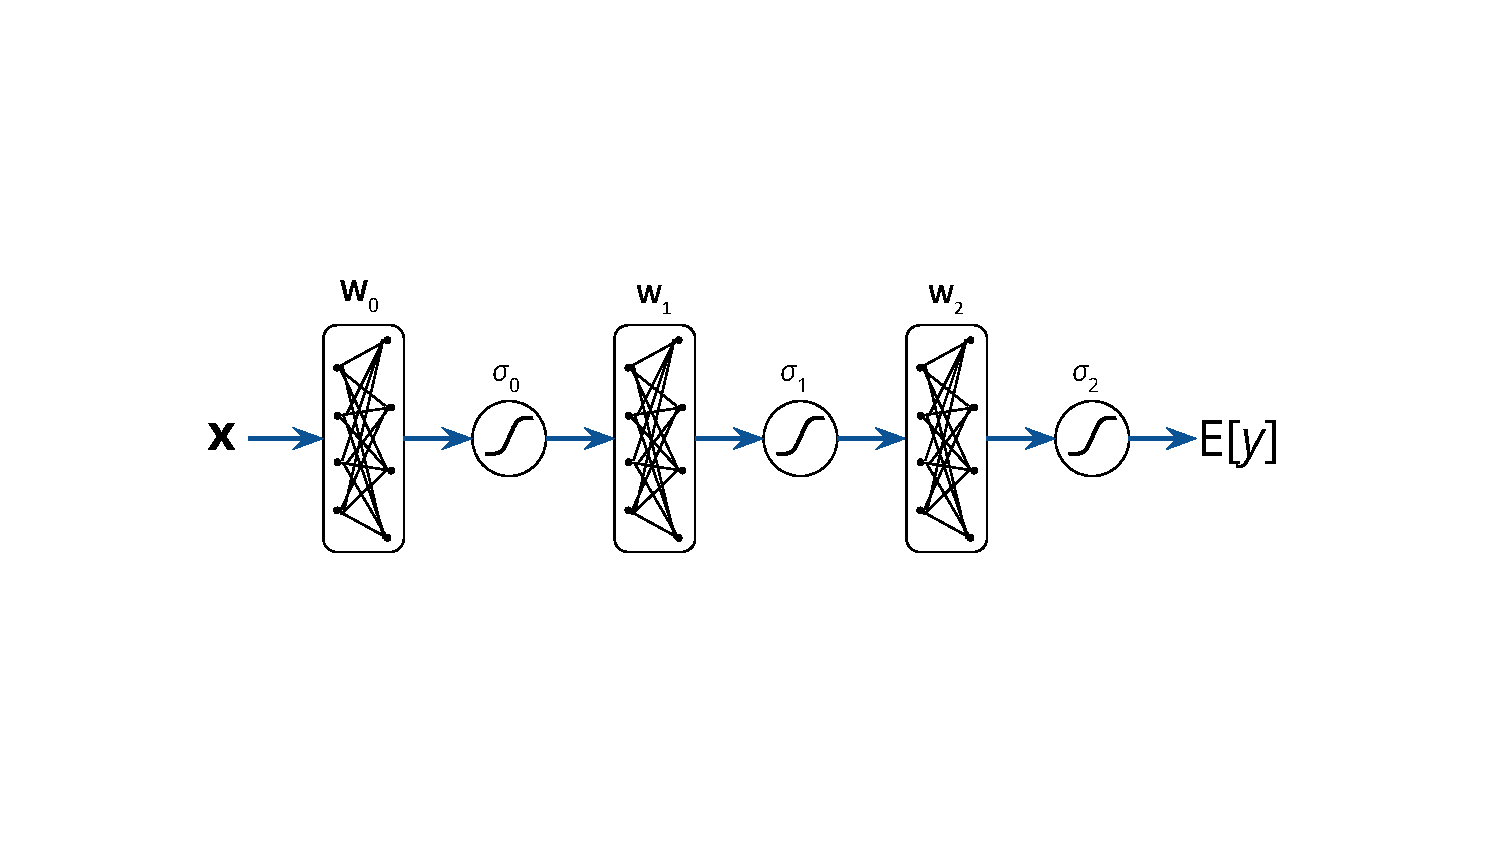
\includegraphics[page=1, width=\pagewidth]{assets/pictures.pdf}
%             };
% \end{tikzpicture}
% \end{frame}


\end{document}
